\documentclass[12pt,oneside]{memoir}

\usepackage[biblatex]{matfmaster}
\usepackage{listings}

\definecolor{bgColor}{rgb}{0.9, 0.9, 0.9}

\lstnewenvironment{code}[2]
{\renewcommand\lstlistingname{Код}\lstset{
		caption={#1},
		float=htpb,
		label={#2},
		captionpos=b,
		frame=single,
		frameshape={RYR}{Y}{Y}{RYR},
		backgroundcolor=\color{bgColor},
		morekeywords={module, func, param, result, export, if, then, else, var, function, return, for, let},
		tabsize=2
	}
}{}

\graphicspath{ {img/} }

\bib{master}

\autor{Сретен Ковачевић}

\naslov{v8 - имплементација неоптимизујућег WebAssembly компилатора за MIPS архитектуру}

\godina{2018}

\mentor{др Филип \textsc{Марић}, ванредни професор\\ Универзитет у Београду, Математички факултет}

\komisijaA{др Милена \textsc{Вујошевић-Јаничић}, ванредни професор\\ Универзитет у Београду, Математички факултет}

\komisijaB{др Милан \textsc{Банковић}, доцент\\ Универзитет у Београду, Математички факултет}

\apstr{
}

\kljucnereci{}

\begin{document}

\frontmatter

\naslovna

\komisija

\posveta{}

\apstrakt

\tableofcontents*

\mainmatter

\chapter{Увод}

\chapter{Архитектура \textit{MIPS}}

У овој глави је описана архитектура \textit{MIPS} процесора. У поглављу \ref{chp:CR} су описане архитектура
процесора \textit{CISC} (скраћено од енгл. \textit{Complex Instruction Set Computing}) и \textit{RISC} (скраћено од
енгл. \textit{Reduced Instruction Set Computing}) и њихове разлике, а у поглављу \ref{chp:MIPS} \textit{MIPS}
архитектура. У поглављима \ref{chp:INS} и \ref{chp:REG} описане су инструкције и регистри \textit{MIPS} архитектуре.
У поглављу \ref{chp:PIPE} описан је механизам проточне обраде и њена имплементација на \textit{MIPS} архитектури, а у
поглављлу \ref{chp:DELAY} је представљен слот закашњења. Поглавље \ref{chp:ENDIANNESS} описује на који начин \textit{MIPS}
архитектура води рачуна о редоследу бајтова у меморији.

\section{\textit{CISC} и \textit{RISC} архитектура} \label{chp:CR}

Архитектура у рачунарству представља спој организације (начин комуникације међу различитим деловима рачунара),
хардвера (примена конкретних логичких кола) и скуп инструкција и регистара \textit{ISA} (скраћено од енгл.
\textit{Instruction Set Architecture}) \cite{ARCH}. Да би разумели разлику између \textit{CISC} (скраћено од енгл.
\textit{Complex Instruction Set Computing}) и \textit{RISC} (скраћено од енгл. \textit{Reduced Instruction Set
Computing}) архитектуре довољно је да посматрамо последњу ставку.

Процесори дизајнирани по \textit{CISC} архитектури карактеришу се великим бројем инструкција које су на раслопагању
програмеру. Овим дизајном се смањује број наредби у програму, по цену броја циклуса по инструкцији. Смањењем броја
инструкција по програму постиже се мања потрошња меморије \cite{CR}. Инструкције често имају различиту дужину
записа, а могу и обављати неколико независних задатака. Оваква архитектура захтева сложен хардвер, што може довести
до потешкоћа у разумевању и програмирању оваквих чипова. Пружају могућност великог броја различитих начина
адресирања. Овакви процесори се користе на личним рачунарима, радним станицама и серверима. Типичан пример је
\textit{Intel x86} серија процесора.

\textit{RISC} архитектура користи високо оптимизован скуп инструкција. Мотив је супротан у односу на мотив
\textit{CISC} архитектуре. Смањује се број циклуса по инструкцији, али се зато добија мањи број инструкција, те је
потребан већи број инструкција по програму. Јединствена карактеристика \textit{RISC} архитектуре је проточна обрада
(енгл. \textit{Pipelining}). Проточна обрада се постиже преклапањем извршавања већег броја инструкција. Захвањујући
томе постижу се боље перформансе у поређењу са \textit{CISC} процесорима \cite{CR}. Како је број инструкција које су
подржане мали, имплементација самог чипа је знатно једноставнија и јефтинија. Подржана су четири начина адресирања:
регистарско, \textit{PC}-релативно, псеудо-директно и базно. Процесори \textit{RISC} архитектуре се користе у
наменским уређајима (енгл. \textit{embedded}) и примери су \textit{ARM} и \textit{MIPS}.

\section{\textit{MIPS}} \label{chp:MIPS}

\textit{MIPS} је представник \textit{RISC} архитектуре, настао средином осамдесетих година двадесетог века на
Станфорд универзитету. Група студената, предвођена Џоном Хенесијем, је истраживала рад \textit{RISC} процесора и
открила да се бољом применом проточне обраде, која је до тад била недовољно искоришћена, може доћи до бржих
процесора на мањем чипу. \textit{MIPS} је током година успео да се одржи на тржишту, али и да сачува епитет једне од
најједноставнијих архитектура \cite{SMR}.

Процесори из \textit{MIPS} породице успели су да пронађу примену у наменским уређајима. Могу се наћи у мобилним
уређајима, мрежним уређајима, сет-топ боксовима, паметним телевизорима. Све претходно наведене примене захтевају
покретање апликација које захтевају интензивна израчунавања (процесирање слика и видеа, анализа података,
интеракција међу субјектима, итд.).

\section{Инструкције} \label{chp:INS}

У \textit{MIPS} асемблерском језику све инструкције су једнаке дужине 32 бита. Могу се поделити у следеће групе
\cite{ISA}:

\begin{itemize}
	\item аритметичке: сабирање, одузимање, множење, дељење
	\item логичке: и, или, шифтовање
	\item приступ меморији: учитавање, записивање у меморију
	\item гранања и скокови
	\item контролне
\end{itemize}
На основу типова операнада, инструкције се могу поделити у три типа \cite{SMR}:

\textbf{R} - Инструкције које као операнд очекују регистре. Представљају се у следећем формату:

$$
OP\ rd, rs, rt
$$
$OP$ представља ознаку инструкције, $rd$ је регистар за смештање резултата, док су регистри $rs$ и $rt$ операнди.
Неки од примера ових инструкција су:
\begin{itemize}
	\item \textit{jr} - скакање на адресу смештену у регистру
	\item \textit{slt} - поставља 1 у регистар уколико је први аргумент мањи од другог
	\item \textit{addu} - смештање у регистар збира аргумената, посматрајући аргументе као неозначене целе бројеве
\end{itemize}

\textbf{I} - Инструкције које као операнде имају регистар и константну вредност, у облику специјалне вредности која
је уписана у инструкцију (енгл. \textit{Immediate}), представљају се форматом:

$$
OP\ rd, rs, Imm
$$
$OP$ представља ознаку инструкције, $rd$ је регистар за смештање резултата, $rs$ први операнд (регистар), а $Imm$
представља константу која је други операнд. Константа може имати највише 16 бита. Примери ових инструкција су:
\begin{itemize}
	\item \textit{lw} - учитавање вредности са адресе $rs+Imm$ у одредишни регистар
	\item \textit{sw} - смештање вредности из одредишног регистра на адресу $rs+Imm$
	\item \textit{beq} - гранање уколико је вредност у регистру једнака константи
	\item \textit{addiu} - смештање у регистар збира вредности из регистра и константе
\end{itemize}

\textbf{J} - Инструкције које се користе при скоковима. Представљају се следећим форматом:

$$
j\ label
$$
Постоје две инструкције овог типа, а то су \textit{j} и \textit{jal}. Код прве инструкције (енгл. \textit{Jump}) се
ток извршавања пребацује на позицију \textit{label}, исто се дешава и са другом инструкцијом (енгл. \textit{Jump and
link}), али се и адреса наредне инструкције уписује у \textit{\$ra} регистар. Ове инструкције прихватају највеће
константе, које су дужине 26 бита, што је оправдано великим бројевима којим се представљају адресе.

\section{Регистри} \label{chp:REG}

Регистри представљају малу, веома ефикасну меморију која се налази у процесору. \textit{MIPS} инструкције могу као
аргументе да примају једино регистре и специјалне константе.У \textit{MIPS} архитектури постоје 32 регистра опште
намене, од којих два имају другачије понашање \cite{SMR}:

\textbf{\$0} - Увек враћа нулу, без обзира шта се у њега уписује

\textbf{ra} - Користи се за смештање адресе повратка из функције приликом коришћења \textit{jal}
инструкције
Сви остали регистри могу се равноправно користити у инструкцијама (чак се и регистар \$0 може користити, али ће ре
резултат у том случају бити занемарен).

У наставку ће бити описани регистри, као и њихово препоручено коришћење:

\textbf{at} - Резервисан за псеудоинструкције које генерише асемблер.

\textbf{v0, v1} - Користе се за смештање целобројних повратних вредности функција. Уколико се резултат не може
сместити у два регистра, компилатор ће резултат сместити у меморију, а адресу у ове регистре.

\textbf{a0 - a3} - Користе се за смештање прва четири целобројна аргумента при позиву функција. Остали се смештају
на стек.

\textbf{t0 - t9} - Привремени регистри, није потребно рестаурирати вредност након коришћења.

\textbf{s0 - s7} - Садржај ових регистара мора остати непромењен након сваке функције, што се постиже привременим
чувањем њиховог садржаја на стеку уколико се користе. Дужност да сачува њихову вредност има позвана функција (енгл.
\textit{callee saved registers}).

\textbf{k0, k1} - Резервисани за системе прекида оперативног система, иначе се ретко користе.

\textbf{gp} - Има два начина примене. Уколико се ради о коду који не зависи од позиције (енгл. \textit{Position
Independent Code} скраћено \textit{PIC}), овај регистар показује на табелу показивача (енгл. \textit{Global Offset
Table}). Уколико је у питању регуларан код, показује на средину у статичкој меморији. На тај начин се помоћу једне
инструкције може приступити било ком податку који је 32KB лево или десно од њега. Овај регистар не користе сви
системи за компилацију и сва окружења за извршавање.

\textbf{sp} - Показивач на стек. Стање стека је потребно експлицитно ажурирати, те се инструкције за одржавање
показивача на стек углавном генеришу на почетку и на крају функција. Како стек расте надоле, на почетку функције се
поставља на најнижу тачку до које ће стек расти.

\textbf{fp} - Показивач на стек оквир. Користи се од стране функције, за праћење стања на стеку. Уколико се при
превођењу не може одредити на коју вредност да се постави \textbf{sp} регистар, променљивим на стеку се приступа
помоћу овог регистра.

\textbf{ra} - Подразумевани регистар за смештање адресе повратка из функције. Овакво понашање је подржано кроз
одговарајуће инструкције скока. Ово је разлика у односу на \textit{x86} архитектуру, где се адреса повратка смешта
на стек. Функције се углавном завршавају наредбом \textit{jr \$ra}. Иако се може користити и било који други
регистар, то се не препоручује због оптимизација које врши процесор у случају коришћења овог регистра. Функције које
позивају друге функције морају сачувати његову вредност.

\section{Проточна обрада} \label{chp:PIPE}

Проточна обрада (енгл. \textit{pipelining}) почива на чињеници да различите фазе извршавања користе различите
ресурсе. Уколико имамо систем у ком је свака фаза једнаке дужине, добили би систем код ког би на крају завршетка
фазе за једну инструкцију у ту фазу ушла следећа инструкција \cite{SMR}. Да би овакав систем био могућ, процесори
\textit{RISC} архитектуре бирају минималан скуп инструкција које имају приближно исто време извршавања у свакој
фази. Такође, инструкције су исте дужине како би се осигурало да је фаза декодирања идентична у свакој фази. Оваква
конфигурација може се видети и у \textit{MIPS} архитектури \cite{SMR}.

Како би проточна обрада била ефикасна користи се кеш меморија, чиме се убрзавају приступи меморији. Кеш меморија је
мала, веома брза, локална меморија у којој се налази копија података из меморије \cite{SMR}. У кешу се чувају подаци
које је процесор најскорије користио, док се најстарији подаци преписују (уколико је кеш попуњен). Када процесор
у кешу не пронађе потребне податке ("промашај кеша", дешава се у 10\% случајева), тада се приступа меморији.

Код \textit{RISC} архитектуре, кеш је уско повезан за процесор и активно се користи за имплементацију проточне
обраде, док се код \textit{CISC} архитектуре кеш посматра као део меморијског система. \textit{MIPS} има одвојен кеш
података и инструкцијски кеш, што омогућава симултано читање инструкција и уписивање или читање података.

\textit{MIPS} инструкције су подељене у пет фаза, и трајање сваке фазе је фиксирано. Прва, трећа и четврта фаза
трају по један такт процесора, док друга и пета захтевају пола такта за своје извршење \cite{SMR}. У наставку је
описана свака од фаза.

\begin{enumerate}
	\item Дохватање инструкције из инструкцијског кеша и њено декодирање
	\item Читање садржаја наведених регистара
	\item Извршавање аритметичко/логичких операција у једном такту (операције у покретном зарезу, множење и дељење су
	сложеније и раде се другачије)
	\item Дохватање и уписивање у меморију. У 75\% случајева инструкције не раде ништа у овој фази, али она постоји
	да не би више инструкција чекало на приступ кешу података
	\item Резултат операције се уписује у одредишни регистар
\end{enumerate}

\section{Слот закашњења} \label{chp:DELAY}

Слот закашњења (енгл. \textit{Delay slot}) је најосетнији ефекат проточне обраде из угла програмера. Због структуре
проточне обраде на \textit{MIPS} архитектури (која је описана у поглављу \ref{chp:PIPE}), у тренутку када наредбе
гранања или скока дођу до фазе извршавања, рад на наредној инструкцији ће већ бити започет, иако је ток извршавања
потенцијално промењен. Започета инструкција се извршава без обзира на исход наредбе промене тока извршавања и на тај
начин се започети посао не одбацује.

Како би се постигло да се у слоту закашњења не појави више од једне инструкције, наредбе гранања имају посебно
понашање при ком се већ после пола такта у фази извршавања аритметичко/логиких операција зна где ће се извршавање
наставити. Како и друга фаза траје пола такта, овим смо обезбедили да само једна инструкција може доспети до прве
фазе, за чије обављање је потребан један такт. Оваква конфигурација пружа могућност програмеру или компилатору да
промени редослед инструкција у програму и тако неко израчунавање смести у слот закашњења \cite{SMR}.

Упркос уштеди коју слот закашњења може да донесе, он представља и потенцијални ризик. Посебно треба истаћи условна
гранања, у којима нека операција не треба да буде извршена у оба случаја. Некад је безбедније (или једино исправно)
оставити у слоту закашњења инструкцију \textit{nop}.

Још једна последица проточне обраде је и слот закашњења учитавања (енгл. \textit{load delay slot}). Подаци дохваћени
\textit{load} инструкцијом постају расположиви тек након инструкције која следи иза ње. Стога се њен резултат не
може користити у следећој инструкцији. Модерни процесори имају механизам блокирања резултата \textit{load}
инструкције. Уколико резултат проба да се искористи у следећој инструкцији, процесор ће зауставити извршавање док
резултат не буде спреман. На ранијим верзијама такав код је имао недефинисано понашање \cite{SMR}.

% TODO: Dodati poglavlje o Endianness-u.
\section{Редослед бајтова} \label{chp:ENDIANNESS}

\chapter{WebAssembly}

\textit{WebAssembly} (скраћено \textit{Wasm}) је безбедан и преносив код ниског нивоа. Дизајниран је са
идејом да обезбеди ефикасно извршавање и компактну репрезентацију. Главни циљ му је да омогући функционисање
апликација високог нивоа на Вебу, али и да не прави никакве претпоставке о окружењу нити уводи нове функционалности,
што би га чинило погодним за коришћење у оквиру других окружења \cite{WASMS}. У овој глави ће бити описан
\textit{WebAssembly} и његове карактеристике. У поглављу \ref{chp:SUPP} ће бити приказан развој језика и заступљеност, а
у поглављу \ref{chp:DESIGN} ће бити приказан дизајн \textit{WebAssembly}-ja, као и карактеристике које са њим долазе.
У поглављу \ref{chp:STRUCT} је описана његова структура, док је у поглављу \ref{chp:PHASES} је дат приказ семантичких
фаза. У поглављу \ref{chp:JSA} дат је преглед могућности које пружа \textit{JavaScript} за коришћење
\textit{WebAssembly}-ja.

\section{Развој и подршка} \label{chp:SUPP}

\textit{WebAssembly} пројекат је започео као \textit{W3C CG} (скраћено од енгл. \textit{World Wide Web Consortium Community Group}),
29. aприла 2015. године \cite{WASMCG}. У групу су се временом укључили произвођачи 4 најпопуларнија прегледача, \textit{Mozilla},
\textit{Microsoft}, \textit{Google} и \textit{Apple}. Технологије које су делимично биле узор и сматрају се претечом су \textit{asm.js} и
\textit{Google Native Client}. За мање од годину дана, ове компаније су имале спреман прототип имплементације
подршке за \textit{WebAssembly} у својим прегледачима \cite{WASMEXP}, док су се прве верзије прегледача са подршком на тржишту нашле у току
2017. године.

\textit{C/C++} апликације могу врло лако превести на \textit{WebAssembly}, a затим и покретати унутар прегледача.
Тако је  могуће користити разне библиотеке већ написане у овим језицима, као што су стандардна библиотека, \textit{OpenGL} и
\textit{SDL} за графичко програмирање, \textit{pthread} за вишенитно програмирање. Ове библиотеке користе инфраструктуру ниског
нивоа које обезбеђује \textit{WebAssembly}, док користе интерфејс других сервиса. Тако се, на пример, \textit{OpenGL} извршава помоћу
\textit{WebGL}, док се уместо системских позива за добијање времена и датума ти позиви прослеђују самом прегледачу и користе се његови
унутрашњи механизми \cite{WASMC++}.

Подршка целе заједнице дала је одличан замајац даљем развоју пројекта и његовом широком прихватању. Убрзо су се појавили и први примери
који су за циљ имали да прикажу моћ новог кода. Један такав пример је и мала демонстрација у виду игре на \textit{Unity} платформи, користећи \textit{WebGL}
библиотеку \cite{GAME}. Изглед игре приказан је на слици \ref{img:TANKS}. Уколико прегледач подржава \textit{WebAssembly}, игра се покреће помоћу њега, док ће,
у супротном, бити покренута \textit{asm.js} верзија игре.

\begin{figure}
\begin{center}
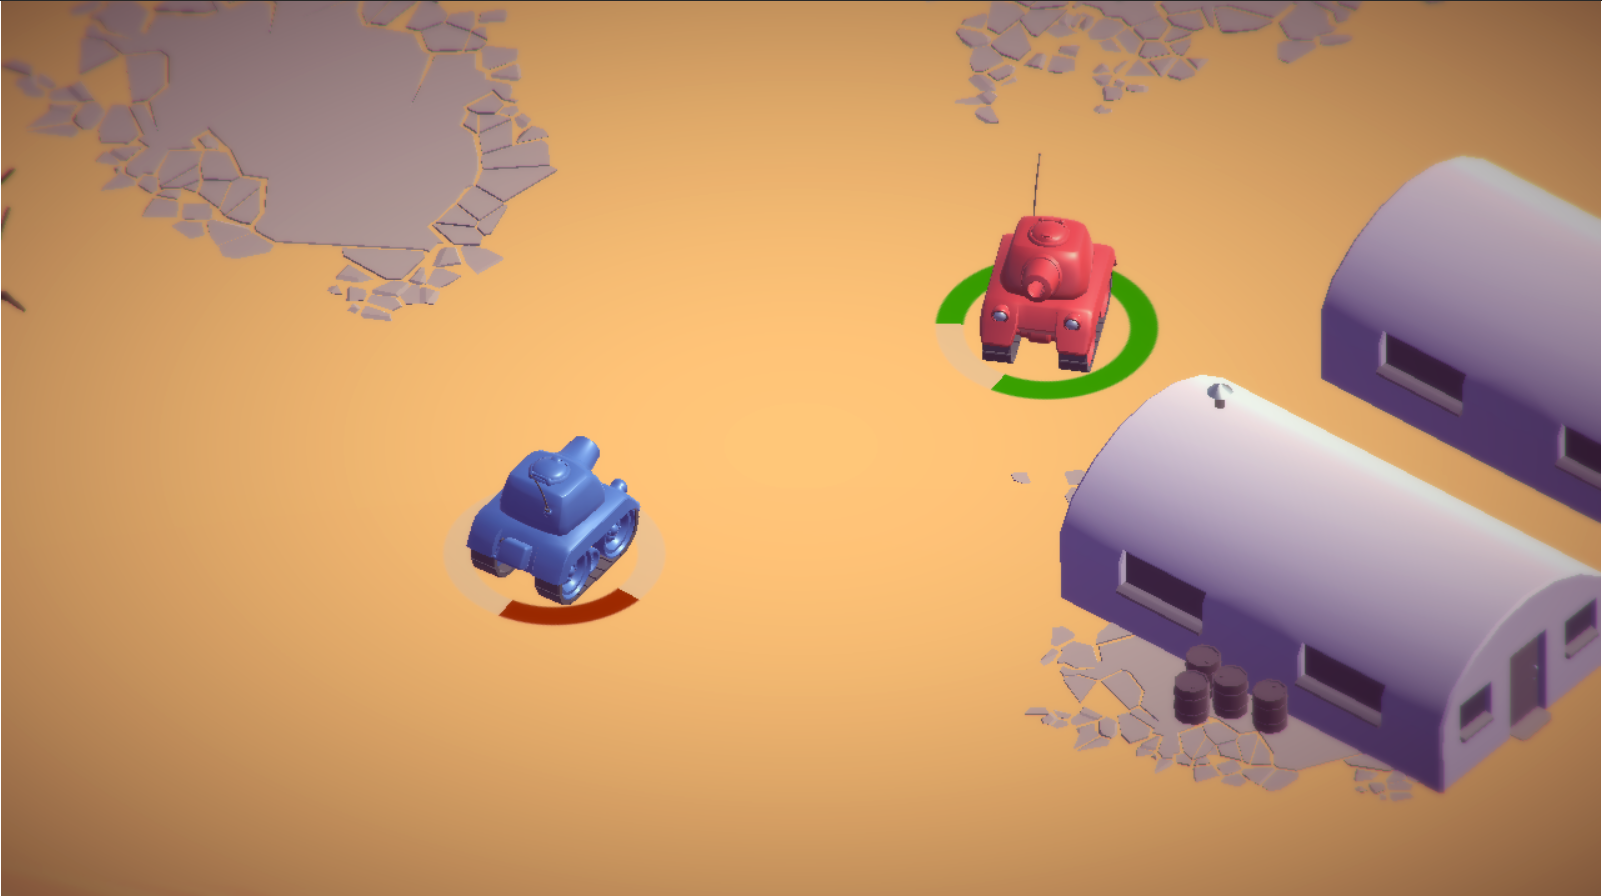
\includegraphics[scale=0.2]{tanks_demo}
\caption{Приказ видео игре}
\label{img:TANKS}
\end{center}
\end{figure}

Брзо се отишло и корак даље, те су се тако појавили покушаји да се врло сложене и захтевне апликације покрену у прегледачу користећи \textit{WebAssembly}.
Пројекат који је добио највећу медијску пажњу и покушај да се популарна игра \textit{Doom 3}. У тренутку њеног појављивања, 2004. године, била је једна од најзахтевнијих
игара и представљала је велики залогај за рачунаре тог времена, док се њена графика и за данашње стандарде сматра врло квалитетном. Уз све то, и чињеницу да је у питању игра
отвореног кода, постала је идеалан кандидат да се заиста тестирају могућности које пружа \textit{WebAssembly}. Иако и даље у развоју, игра се испешно извршава и тренутно
показује да је верзија која се покреће кроз прегледач користећи \textit{WebAssembly} за 40-60\% спорија од игре која се извршава директно на машини. Иако резултат сам
по себи не делује импресивно, треба додати да је то и до 3 пута брже у односу на верзију која корити само \textit{Javascript} \cite{D3WASM}.

\section{Дизајн} \label{chp:DESIGN}

Пред \textit{WebAssembly} су постављени одређени циљеви у погледу дизајна. Два основна циља су брза, безбедена и
преносива семантика и ефикасна и преносива репрезентација. Оба циља са својим испуњењем језику пружају
карактеристике неопходне да се постигне жељени ниво перформанси.

Из угла семантике \textit{WebAssembly} je \cite{WASMS}:

\begin{itemize}
	\item Брз - извршава се ефикасношћу која тежи ефикасности језика нижег нивоа (енгл. \textit{native}), користећи
	предности савременог хардвера
	\item Безбедан - код се валидира и извршава у меморијском сефу, заштићеном окружењу које спречава угрожавање
	података или упаде
	\item Добро дефинисан - потпуно и прецизно дефинише исправне програме и њихово понашање на начин који је лако
	разумети, како формално тако и неформално
	\item Хардверски независтан - може се превести на свим архитектурама, персоналним и преносивим рачунарима и
	наменским уређајима
	\item Језички независтан - не фаворизује одређени језик вишег нивоа, стил програмирања или објектни модел
	\item Платформски независтан - може бити уграђен у прегледач, представљати самосталну виртуелну машину или
	представљати део неког већег окружења
	\item Отворен - програми могу комуницирати са окружењем користећи једноставне методе
\end{itemize}
Посматрајући репрезентацију \textit{WebAssembly}-ja, можемо закључити да је \cite{WASMS}:

\begin{itemize}
	\item Компактан - бинарни формат се брзо преноси захваљујући запису који је краћи и од обичног текста и од кода
	на језику ниског нивоа
	\item Модуларан - програм се може поделити на мање целине које се могу слати, кеширати и користити независно
	\item Ефикасан - може се декодирати, валидирати и компилирати у једном пролазу, како са \textit{JIT} (скраћено
	од 
	енгл. \textit{Just-in-time}) тако и са \textit{AOT} (скраћено од енгл. \textit{Ahead-of-time}) компилацијом
	\item Проточан (енгл. \textit{streamable}) - омогућује да декодирање, валидација и компилација почну пре него
	што
	су сви подаци на располагању
	\item Погодан за паралелизацију (енгл. \textit{parallelizable}) - допушта да декодирање, валидација и компилација буду
	издељени у више независних паралелних задатака
	\item Преносив - не прави претпоставке о архитектури које нису широко распрострањене међу модерним хардвером
\end{itemize}

\section{Структура} \label{chp:STRUCT}

\textit{WebAssembly} кодира језик ниског нивоа, који је налик на асемблер. Његову структуру чине \cite{WASMS}:

\begin{itemize}
	\item Вредности
	\item Инструкције
	\item Замке (енгл. \textit{Traps})
	\item Функције
	\item Табеле
	\item Линеарна меморија
	\item Модули
	\item Уграђивач (енгл. \textit{Embedder})
\end{itemize}
У наставку ће бити описан сваки од елемената структуре.

\subsection{Вредности}

У оквиру \textit{WebAssembly}-ja постоје четири типа вредности. То су целобројне вредности и бројеви у покретном
зарезу (имплементирани по стандарду \textit{IEEE 754-2008)}, оба у 32-битној и 64-битној варијанти. 32-битне
целобројне вредности се користе и за репрезентацију истинитосних вредности (енгл. \textit{boolean}) и меморијских
адреса. На располагању су све уобичајене операције над овим типовима, као и конверзије међу њима. Не постоји разлика
између означених и неозначених целих бројева, већ се на основу конкретне операције одлучује како ће се број
посматрати \cite{WASMS}.

\subsection{Инструкције}

Рачунски модел је заснован на принципима стек машине. Код се састоји од низа инструкција које се редом извршавају.
Инструкције врше промене над подацима који се налазе на имплицитном стеку операнада и могу се поделити у две основне
категорије. Једноставне инструкције са стека узимају аргумент и резултат смештају назад на стек. Контролне
инструкције мењају ток извршавања програма. Програм је добро структуиран, односно подељен у блокове, петље и условне
кодове и наредбе гранања могу да гађају само неке од ових структура \cite{WASMS}.

\subsection{Замке}

Неке инструкције, под одговарајућим условима, могу изазвати замку (енгл. \textit{trap}), које прекидају извршавање
програма. \textit{WebAssembly} не поседује механизам за обраду замки, већ се оне прослеђују окружењу, где се хватају
и обрађују на одговарајући начин \cite{WASMS}.

\subsection{Функције}

Код је подељен у одвојене функције. Свака функција прима низ вредности као параметре и враћа низ вредности као
резултат\footnote{У тренутној имплементацији може се вратити само један резултат.}. Функције се могу међусобно
позивати, укључујући и рекурзивне позиве. Функције могу декларисати локалне променљиве које се могу користити попут
виртуелних регистара \cite{WASMS}. Пример функције која враћа факторијел броја дат је у оквиру кода \ref{cd:MOD}.


\subsection{Табеле}

Табела представља низ вредности неког типа. На тај начин се допушта програму да помоћу индекса индиректно приступи
елементу. Тренутно, једини подржани тип је референца на функцију. Захваљујући томе, програм може позивати функције
користећи само индекс табеле. Ово опонаша показивачe на функције \cite{WASMS}.

\subsection{Линеарна меморија}

Линеарна меморија је непрекидан, променљив низ сирових бајтова. Таква меморија има иницијалну величину, али се може
динамички проширити. Програм може учитати или уписати вредност у меморију на адресу било ког бајта (укључујући и
непоравнату). Уколико се покуша приступ ван тренутних граница меморије, замка ће бити активирана \cite{WASMS}.

\subsection{Модули}

\textit{WebAssembly} у свом бинарном запису узима облик модула. Модул садржи дефиниције функција, табела, и линеарне
меморије. Такође, може садржати и глобалне променљиве и константе. Дефиниције могу бити увезене тако што ћемо
навести модул из ког увозимо и име дефиниције коју увозимо заједно са одговарајућим типом. Опционо, неке дефиниције
могу бити извезене под једним или више различитих имена. Осим дефиниција, могу се додати иницијализациони подаци за
меморије и табеле. Могу садржати и почетне функције, чије извршавање се одвија аутоматски \cite{WASMS}. У коду
\ref{cd:MOD} дат је пример једноставног модула који извози функцију.

\begin{code}{Пример модула који извози функцију за рачунање факторијела}{cd:MOD}
(module
	(func $fact (param $0 i32) (result i32)
		get_local $0
		i32.const 0
		i32.eq
		(if (result i32)
			(then
				i32.const 1
			)
			(else
				get_local $0
				get_local $0
				i32.const 1
				i32.sub
				call $fact
				i32.mul
			)
		)
	)
	(export "factorial" (func $fact))
)
\end{code}

\subsection{Уграђивач}

Имплементација \textit{WebAssembly}-ja је углавном уграђена (енгл. \textit{embedded}) у окружење домаћина. То
окружење одређује како ће модули бити учитани, како су увози доступни и како се приступа извезеним дефиницијама.
Детаљи зависе од окружења и нису одређени структуром самог језика \cite{WASMS}. Конкретни примери уграђивача биће
приказани касније.

\section{Семантичке фазе} \label{chp:PHASES}

Семантика је подељена у три фазе. За сваки део језика постоји одговарајућа фаза, а оне су \cite{WASMS}:

\textbf{Декодирање} - \textit{WebAssembly} модули се шаљу у бинарном облику. Модул представљен кодом \ref{cd:MOD}
у бинарном формату заузима 62 бајта и његов хексадекадни запис\footnote{Хексадекадни запис добијен коришћењем скупа
алата \textit{WABT} (скраћено од енгл. \textit{WebAssembly Binary Toolkit}) \cite{WABT}.} дат кодом \ref{cd:HEX}.
Декодирање је процес који форматира и конвертује бинарни облик у интерну репрезентацију модула. Интерна
репрезентација може бити у облику апстрактне синтаксе, али и конкретан машински код.

\begin{code}{Хексадекадни запис модула}{cd:HEX}
00 61 73 6d 01 00 00 00 01 06 01 60 01 7f 01 7f
03 02 01 00 07 0d 01 09 66 61 63 74 6f 72 69 61
6c 00 00 0a 19 01 17 00 20 00 41 00 46 04 7f 41
01 05 20 00 20 00 41 01 6b 10 00 6c 0b 0b
\end{code}

\textbf{Валидација} - Декодирани модул мора бити валидан. Ова фаза проверава услове добре дефинисаности како би се
осигурало да је модул исправан и безбедан. Прецизније, врши се провера типова функција, као и низ инструкција које
јој припадају како би се утврдило да је стек операнада конзистентно коришћен.

\textbf{Извршавање} - Уколико су прве две фазе успешно окончане, модул се може извршити. Сама фаза извршавања се
састоји од две подфазе:

\begin{itemize}
	\item Инстанцирање (енгл. \textit{Instantiation}) - Инстанца модула је његова динамичка репрезентација, са
	сопственим стањима и стеком извршавања. У овој	фази се извршава тело модула, све увезене дефиниције,
	иницијализују се глобалне променљиве, меморије, табеле и активира се почетна функција (уколико је дефинисана).
	Враћа примерке извоза модула.
	\item Позивање (енгл. \textit{Invocation}) - Jедном када је фаза инстанцирања завршена, њен резултат се може
	користити да се позивају извезене функције из претходно инстанцираног модула. Функцијама се прослеђују
	одговарајући аргументи, а као резултат се добија резултат њиховог извршавања.
\end{itemize}
Фазе инстанцирања и позивања су операције које одређује окружење домаћина.

\section{JavaScript API} \label{chp:JSA}

Као што је речено у секцији \ref{chp:DESIGN}, \textit{WebAssembly} може бити део неког већег система. Данас се
\textit{WebAssembly} модули углавном користе у већ постојећим \textit{Javascript} апликацијама.
Иако постоји идеја да се у будућности \textit{WebAssembly} модули учитавају попут било ког \textit{Javascript}
модула, данас то није случај и стога је потребан посебан интерфејс.

Тај интерфејс је дужан да обезбеди 3 основна корака \cite{WASMJS}:

\begin{enumerate}
	\item Смештање бајт-кода у типизирани \textit{ArrayBuffer}
	\item Превођење бајт-кода у \textit{WebAssembly.Module} објекат
	\item Инстанцирање објекта типа \textit{WebAssembly.Module} уз увожење и извожење потребних елемената.
\end{enumerate}

У наставку ће бити приказан пример који показује употребу оваквог интерфејса за увоз и извоз функција. Нека је дат \textit{WebAssembly} модул
\ref{cd:wasm_simple}, зовимо га у наставку \textit{simple.wasm} и \textit{Javascript} код \ref{cd:js_simple}.

\begin{code}{\textit{simple.wasm}}{cd:wasm_simple}
(module
	(func $i (import "imports" "i") (param i32))
	(func (export "e")
		i32.const 42
		call $i))
\end{code}

\begin{code}{\textit{Javascript} код који користи модул из \textit{simple.wasm}}{cd:js_simple}
function instantiate(bytes, imports) {
	return WebAssembly.compile(bytes)
	.then(m => new WebAssembly.Instance(m, imports));
}

var importObject = 
	{ imports: { i: arg => console.log(arg) } };

bytes = readbuffer("simple.wasm")
instantiate(bytes, importObject)
.then(instance => instance.exports.e())
\end{code}

\textit{simple.wasm} увози функцију са два нивоа приступних имена (\textit{imports.i}), те и
променљива \textit{importObject} мора да одражава такву структуру. Функција \textit{fetch} добавља код модула из захтева 
пристиглог са мреже, након чега резултат преводимо помоћу \textit{WebAssembly.compile()} метода и инстанцирамо модул прослеђујући бајт-код
и увозни објекат \textit{importObject} помоћу конструктора \textit{WebAssembly.Instance}. Тада, из добијене инстанце можемо позвати
изведену функцију. Резултат овог програма је исписивање броја 42 на стандардни излаз. На овај начин је у потпуности омогућена комуникација
између \textit{Javascript} и \textit{WebAssembly} кода.

Још један битан део \textit{WebAssembly} структуре програма који треба да буде доступан из \textit{Javascript} кода је
линеарна меморија. За \textit{Javascript}, линеарна меморија је \textit{ArrayBuffer} који је променљиве величине. Нова меморија
може бити инстанцирана коришћењем \textit{WebAssembly.Memory()} конструктора, који може примати до 2 аргумента. Први је иницијална
величина меморије, а други максимална дозвољена. Оба аргумента представљају број \textit{WebAssembly} страница, од којих је свака
величине 64 килобајта. Овај објекат садржи елемент \textit{buffer} који је типа \textit{ArrayBuffer}.

Осим креирања, могуће је приступити сваком појединачном бајту користећи оператор []. Над \textit{WebAssembly.Memory}
објектом дозвољена је и операција проширивања меморије помоћу метода \textit{grow}. Као и код функција, меморија може бити и увезена и извезена из модула.
На овај начин, добијамо могућност да у сваком тренутку проверимо или променимо стање меморије, али и да поставимо иницијално стање меморије.

\chapter{V8}

\textit{V8} је \textit{JavaScript} мотор (енгл. \textit{engine}) отвореног кода, написан у jeзику \textit{C++},
развијен од стране компаније \textit{Google}. Осим у оквиру њиховог пројекта \textit{Chromium}, који се користи као основа за многе веб прегледаче,
међу којима је најпопуларнији \textit{Google Chrome}, \textit{V8} je саствни део и \textit{Node.js} пројекта. У поглављу \ref{chp:DEV} биће речи о развоју
\textit{V8 JavaScript} мотора, док ће у поглављу \ref{chp:CHAR} бити представљене његове карактеристике. Оптимизујући компилатор \textit{TurboFan}
биће приказан у поглављу \ref{chp:OPT}. У поглављу \ref{chp:V8WASM} биће приказана подршка за \textit{WebAssembly} унутар \textit{V8}.

\section{Развој} \label{chp:DEV}

Прва званична верзија \textit{V8 JavaScript} мотора појавила се, заједно са првом верзијом \textit{Google Chrome} веб прегледача, у септембру 2008. године. Креатор
овог пројекта је дански програмер Ларс Бак \cite{V8SP}. Првобитна архитектура предвиђала је његову употребу само у оквиру веб прегледача.

\textit{V8} се може покренути на 3 различита оперативна система (\textit{Windows}, \textit{MacOS} и \textit{Linux}), али и на различитим процесорским архитектурама, од којих
су најпопуларнији \textit{x64}, \textit{IA-32}, \textit{ARM} и \textit{MIPS}.

Временом се мењала архитектура \textit{V8} мотора. У тренутку појављивања, она је била врло једноставна. Парсер је од улазног \textit{JavaScript} кода стварао апстрактно
синтаксно стабло, које је било улаз компилатору под називом \textit{Codegen}, чији резултат је био оптимизован код. Архитектура је приказана на слици \ref{img:V8_1}.
Ипак, даљом анализом и развојем, дошло се до закључка да и даље постоји доста простора за нове оптимизације, те се тако променила и архитектура, слика \ref{img:V8_2}.
2010. године \textit{Codegen} замењен је неоптимизујућим компилатором, под називом \textit{Full-Codegen}, који је, осим генерисања, скупљао и информације о извршавању и
прослеђивао их оптимизујућем компилатору, који носи назив \textit{Crankshaft}.

\begin{figure}
\begin{center}
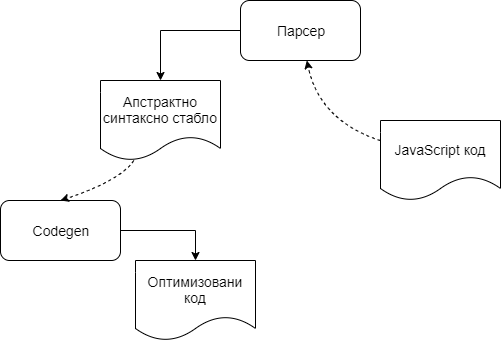
\includegraphics[scale=0.5]{v8_1}
\caption{Архитектура \textit{V8} из 2008. године}
\label{img:V8_1}
\end{center}
\end{figure}

\begin{figure}
\begin{center}
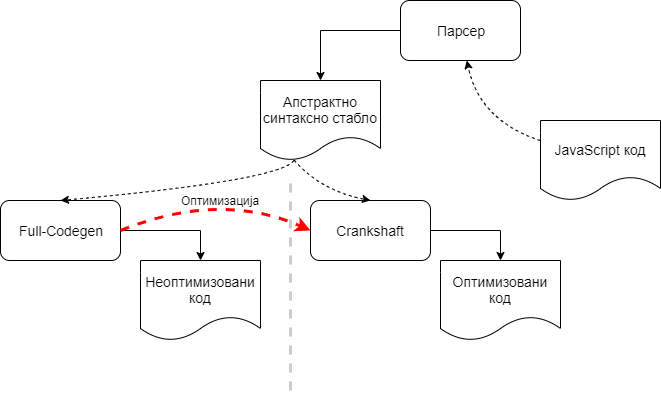
\includegraphics[scale=0.5]{v8_2}
\caption{Архитектура \textit{V8} из 2010. године}
\label{img:V8_2}
\end{center}
\end{figure}

Ова архитектура је само 4 године касније добила новог члана. Нови оптимизујући компилатор, под називом \textit{TurboFan}, представљао је идеју за будућност, са циљем да временом
потпуно одмени \textit{Crankshaft}. Нова архитектура је приказана на слици \ref{img:V8_3}. Да би се транзиција на \textit{TurboFan} у потпуности обавила, био је неопходан још
један део целој слагалици. У питању је интерпретер, под називом \textit{Ignition}. Његовим додавањем, \textit{TurboFan} је могао да престане да користи постојеће компоненте.
Ова архитектура приказана је на слици \ref{img:V8_4} и представља стање из 2016. године. Само годину дана касније, застарели делови архитектуре, \textit{Full-Codegen} и
\textit{Crankshaft}, су уклоњени из кода. Тако је добијена тренутна верзија, приказана на слици \ref{img:V8_5}.

\begin{figure}
\begin{center}
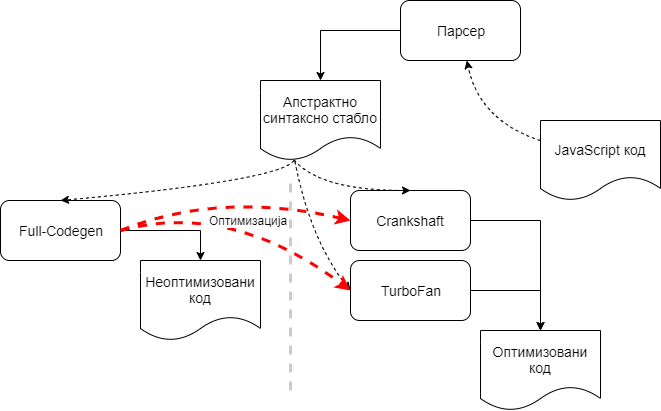
\includegraphics[scale=0.5]{v8_3}
\caption{Архитектура \textit{V8} из 2014. године}
\label{img:V8_3}
\end{center}
\end{figure}

\begin{figure}
\begin{center}
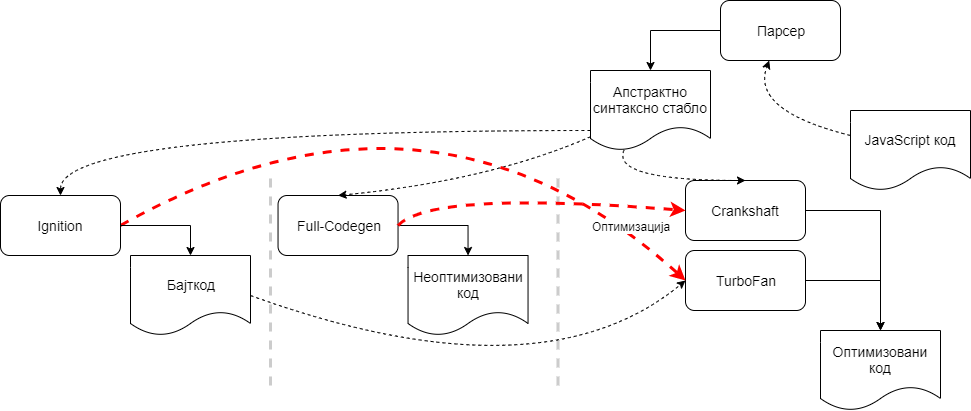
\includegraphics[scale=0.4]{v8_4}
\caption{Архитектура \textit{V8} из 2016. године}
\label{img:V8_4}
\end{center}
\end{figure}

\begin{figure}
\begin{center}
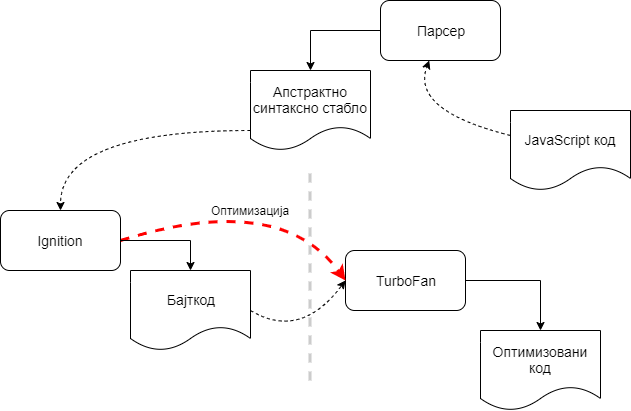
\includegraphics[scale=0.5]{v8_5}
\caption{Архитектура \textit{V8} из 2017. године}
\label{img:V8_5}
\end{center}
\end{figure}

Промене архитектуре које су се догодиле су довеле до тога да \textit{V8} нађе примену и мимо самог прегледача, те је тако постао неизоставни део \textit{Node.js} пројекта.
\textit{V8} се може покренути и као део \textit{C++} апликације, те се убрзо нашао и у другим популарним порјектима, као што су \textit{Couchbase} (\textit{NoSQL} база података),
\textit{Electron} (библиотека за развој корисничких интерфејса) и многи други.

\section{Карактеристике} \label{chp:CHAR}

\textit{V8} је динамички компилатор за језик \textit{JavaScript}. Техника динамичке компилације предвиђа одлагање дела (или свих) оптимизација за фазу извршавања.
Предност оваквог приступа у односу на традиционалан, где се све оптимизације обављају унапред, огледа се у томе што, потенцијално, сваки вид употребе може резултовати
другачије изгенерисаним кодом, оптималнијим за конкретну ситуацију.

Динамичка или \textit{JIT} (скраћено од енгл. \textit{Just-in-time}) техника компилације подразумева следеће елементе:

\begin{itemize}
	\item Профајлер (енгл. \textit{profiler})
	\item Неоптимизујући копмилатор (енгл. \textit{baseline compiler})
	\item Оптимизујући компилатор
\end{itemize}

Профајлер или контролор (енгл. \textit{monitor}) задужен је да прати извршавање кода и води евиденцију о "врућим" деловима кода. Код је "врућ" уколико извршавање
често доводи до истог дела кода. Такви делови кода су погодни за оптимизацију.

Неоптимизујући компилатор је први вид побољшања перформанси. Његово задужење је да изгенерише бајт-код за "врући" део кода. Над таквим бајт-кодом може доћи до мањих оптимизација,
које не захтевају дубљу анализу и могу се брзо испоручити. На пример, неоптимизујући компилатор не прави претпоставке о типовима, већ покрива све могуће случајеве. Тако,
може издвајати сегменте функција у мање функције (енгл. \textit{stubs}). Уколико се овакве функције позивају из неке петље и сваки пут се врши провера типа, убрзање
практично и не постоји. Пример можемо видети у коду \ref{cd:STUB}.
%TODO: Nadji nacin da lepse uneses JS kod.
\begin{code}{Пример функције са петљом}{cd:STUB}
	function acc(array) {
		var result = 0;

		for (let i = 0; i < array.length; i++) {
			result += array[i]
		}

		return result;
	}
\end{code}

Управо је то пример у ком до изражаја долази оптимизујући компилатор. Узимајући у обзир резултате добијене од профајлера, али и бајт-код добијен неоптимизујућим компилатором,
оптимизујући компилатор врши оптимизације у циљу уштеде ресурса. Уколико претпоставимо да је неоптимизујући компилатор изгенерисао мање функције за код из петље из примера \ref{cd:STUB},
знамо да се при сваком пролазу кроз петљу врши провера типа како би се позвала одговарајућа функција. Врло је вероватно да сваки пролазак кроз петљу заправо
има исти тип у оквиру једног пролаза кроз низ. Дакле, уколико би оптимизујући компилатор проширио \textit{stub} изгенерисан од стране неоптимизујућег компилатора
и уместо само тог малог сегмента изгенерисао код за целу функцију, или бар покрива више од саме петље (иако остатак функције не спада нужно у "врући" код),
провера типа би се извукла ван петље.

\section{Оптимизујући компилатор} \label{chp:OPT}

Оптимизујући компилатор који се користи у оквиру \textit{V8} пројекта назива се \textit{Turbofan}. Заснован је на концепту званом "море чворова" (енгл. \textit{Sea-of-nodes}) \cite{SON}.
Овај концепт подразумева употребу једноставног графа за међукод (енгл. \textit{Intermediate Representation}, скраћено \textit{IR}), али, уместо уобичајених графова контроле тока (енгл. \textit{Control-Flow-Graph}
, скраћено \textit{CFG}) и графова тока података (енгл. \textit{Data-Flow-Graph}, скраћено \textit{DFG}), користи се њихова комбинација.

Оваквом комбинацијом графова, тежи се структури која ће задржати повољне карактеристике из оба графа. Оригиналном \textit{DFG} графу додају се информације о контроли тока.
Осим грана зависности података, додају се гране зависности контроле тока. Због својстава које има \textit{CFG} граф, ова структура је погодна за даљу обраду у
циљу добијања крајњег производа, машинског кода. Другим речима, није потребно направити корак у назад зарад лакшег оптимизовања. Такође, добијени граф није стриктно условљен
редоследом чворова, као што је то случај у \textit{CFG} графу.

Са друге стране, карактеристике \textit{DFG} графа, у форми статичке јединствене доделе (енгл. \textit{Static Single Assignment}, скраћено \textit{SSA}), пружају добру стартну позицију
за даље оптимизације, као што су пропагација константи и анализа живости променљивих, али и многе друге. Овакве карактеристике омогућавају лаку манипулацију над чворовима графа.
Најчешће операције над оваквим графом су операције редукције.

Највећи део оптимизација се одвија управо над \textit{Sea-of-nodes} графом. Ипак, једном када се фаза оптимизације заврши, прелази се на традиционалан \textit{CFG} граф.
Управо предностни, као што су, на пример, већа слобода у редоследу чворова у графу, које су погодне за оптимизацију, чине овај граф мање погодним за фазу распоређивања
инструкција (енгл. \textit{Instruction Scheduling}). Веома често је, међу мноштвом потенцијалних распореда инструкција, тешко или немогуће изабрати прави. Стога се примена стриктнијег \textit{CFG}
графа показала успешнијом у овој фази \cite{TFJIT}.

\section{\textit{WebAssembly} подршка} \label{chp:V8WASM}

Као што је поменуто у секцији \ref{chp:SUPP}, сви водећи произвођачи веб прегледача избацили су прототип подршке за \textit{WebAssembly} у току 2016. године, а у току 2017.
и прве званичне верзије са подршком. Такав је случај и са \textit{V8} мотором компаније \textit{Google}.

Донета је одлука да се подршка у оквиру \textit{V8} мотора дода кроз \textit{TurboFan} оптимизујући компилатор. У потпуности је искоришћена структура и функционалност која се користи
за \textit{JavaScript} код, једино је додат нови ниво енкапсулације за чворове изгенерисаног \textit{Sea-of-nodes} графа, како би се сачувале доданте информације неопходне за
\textit{WebAssembly}.

Овакав приступ је довео до тога да се уз минималан посао дође до потпуне подршке и потпуно функционалног компилатора. Ипак, оптимизације које пружа \textit{TurboFan}, осим погодности,
донела је и један велики проблем: брзину превођења. Колико год код изгенерисан \textit{TurboFan} оптимизујућим компилатором био ефикасан, време потребно да тај код
постане расположив представља огроман губитак, чиме се анулира предност која се добија у извршавању, поготову за код који се извршава само једном.

%TODO: Dodaj primer vremena potrebnog za generisanje. Najbolje iskoristiti primer koji je koriscen i u WASM sekciji za Fact.

Такве карактеристике указале су на потребу за неоптимизујућим компилатором. Улога неоптимизујућег компилатора би била да што брже изгенерише валидан код,
а да се тек у наредним итерацијама, по потреби, позива \textit{TurboFan} који би пружио оптималан код и побољшање перформанси у току извршавања.
Тако се, почетком 2018. почело са увођењем неоптимизујућег \textit{Liftoff} компилатора, са циљем да се комплетира подршка за \textit{WebAssembly}.

\chapter{Имплементација}

\chapter{Закључак}

\literatura

\backmatter

\end{document}